\FloatBarrier\section{Auditoría, dependencias y partición reproducible}

\subsection{Contrato de entrada y conservación}
La auditoría parte del CSV original y comprueba que cada identificador de imagen tenga un único archivo en los dos lotes esperados. Se comparan los conjuntos de nombres, se leen dimensiones y contenido decodificable, y se calcula SHA-256 de cada JPEG. Un archivo ausente, una etiqueta fuera de la taxonomía o un identificador repetido detienen la preparación; no se corrigen silenciosamente los datos para lograr que el código continúe.

Las imágenes originales permanecen intactas en \texttt{descargaDataSet/HAM10000}. Desde el archivo \texttt{split.csv} se exportan también las carpetas \texttt{train}, \texttt{val} y \texttt{test} por clase ($224\times224$ sin aumento en disco), \texttt{dataset\_procesado.csv} y \texttt{estadisticas.json} calculado exclusivamente sobre entrenamiento. Durante el experimento, el entrenamiento lee directamente los JPEG originales para evitar doble compresión, sin reutilizar aumentos sintéticos como muestras independientes.

\subsection{Imagen, lesión y paciente}
La auditoría confirma 10\,015 imágenes y 7\,470 lesiones únicas (Figura~\ref{fig:lesiones}). Varias imágenes pueden representar la misma lesión bajo distintas condiciones o aumentos ópticos. En concreto, el análisis de multiplicidad muestra que 5\,514 lesiones (73.8\%) tienen una única toma, 1\,423 (19.0\%) tienen dos tomas, 490 (6.6\%) tienen tres, y 43 lesiones reúnen entre cuatro y seis tomas (34 con cuatro, 5 con cinco y 4 con seis). Si una toma se utiliza para aprender y otra para evaluar, la prueba mediría reconocimiento de la lesión ya vista en lugar de generalización. Por ello se agrupa por \texttt{lesion\_id}.

\begin{tcolorbox}[notaBox,title={Alcance de la independencia garantizada}]
No debe afirmarse independencia por paciente. Un paciente podría aportar más de una lesión y \texttt{HAM10000\_metadata.csv} no incluye un identificador de paciente. El nivel de independencia garantizado por este protocolo es el de \texttt{lesion\_id} y duplicados binarios vinculados por SHA-256.
\end{tcolorbox}

\subsection{Duplicados exactos y similitud visual}
Se detectaron dos registros adicionales cuyo contenido binario coincide exactamente con otro JPEG indexado (\texttt{ISIC\_0024366}/\texttt{ISIC\_0029861} en \texttt{HAM\_0002300} y \texttt{ISIC\_0024777}/\texttt{ISIC\_0029938} en \texttt{HAM\_0001895}, ambos en la clase \texttt{nv}). Se conservan por trazabilidad y quedan confinados en el mismo grupo mediante \textit{Union-Find} (registrado en \texttt{auditoria.json}). Adicionalmente, en una comprobación puntual de sesión (sin script ni reporte independiente persistido en el repositorio), un barrido por parejas sobre miniaturas RGB $16\times 12$ entre todas las muestras con distinto \texttt{lesion\_id} encontró cero pares con $\mathrm{RMSE}<4.5$.

SHA-256 y la comparación de baja resolución descartan igualdad de bytes y copias casi idénticas directas, pero no reemplazan una revisión dermatológica especializada de similitud visual. La documentación y \texttt{auditoria.json} mantienen esta limitación perceptual de forma transparente.

\subsection{Construcción del split fijo}
Se utiliza \texttt{StratifiedGroupKFold} con veinte pliegues, mezcla reproducible y semilla 42. Los pliegues cero a dos forman \texttt{test}; los tres a cinco forman \texttt{val}; los catorce restantes forman \texttt{train}. La estratificación conserva proporciones de clase mientras el agrupamiento mantiene las dependencias juntas \cite{sklearndocs}.

Esta construcción produce aproximadamente 70/15/15, sin prometer porcentajes exactos por imagen porque los grupos no pueden fraccionarse. Los resultados reales son 7\,009 imágenes en \texttt{train} (69.99\%), 1\,503 en \texttt{val} (15.01\%) y 1\,503 en \texttt{test} (15.01\%). La misma asignación se reutiliza en las tres CNN y en Colab. La referencia 80/20 mencionada en orientaciones generales se interpreta como referencial; cualquier otro reparto exigiría fijar un nuevo protocolo antes de experimentar.

\begin{table}[htbp]\centering\normalsize
\setlength{\tabcolsep}{8pt}
\caption{Conteos reales de la partición fija libre de fuga (\textasciitilde 70/15/15) y pesos de clase en entrenamiento.}
\begin{tabularx}{\textwidth}{>{\raggedright\arraybackslash}Xrrrr}\toprule
\textbf{Clase} & \textbf{Train} & \textbf{Val} & \textbf{Test} & \textbf{Peso $w_c$} \\ \midrule
\texttt{akiec} & 228 & 50 & 49 & 4.3916 \\
\texttt{bcc} & 359 & 77 & 78 & 2.7891 \\
\texttt{bkl} & 769 & 165 & 165 & 1.3021 \\
\texttt{df} & 80 & 18 & 17 & 12.5161 \\
\texttt{mel} & 779 & 166 & 168 & 1.2853 \\
\texttt{nv} & 4\,694 & 1\,006 & 1\,005 & 0.2133 \\
\texttt{vasc} & 100 & 21 & 21 & 10.0129 \\
\midrule
\textbf{Total} & \textbf{7\,009} & \textbf{1\,503} & \textbf{1\,503} & --- \\
\bottomrule\end{tabularx}\end{table}


\begin{figure}[htbp]
\centering
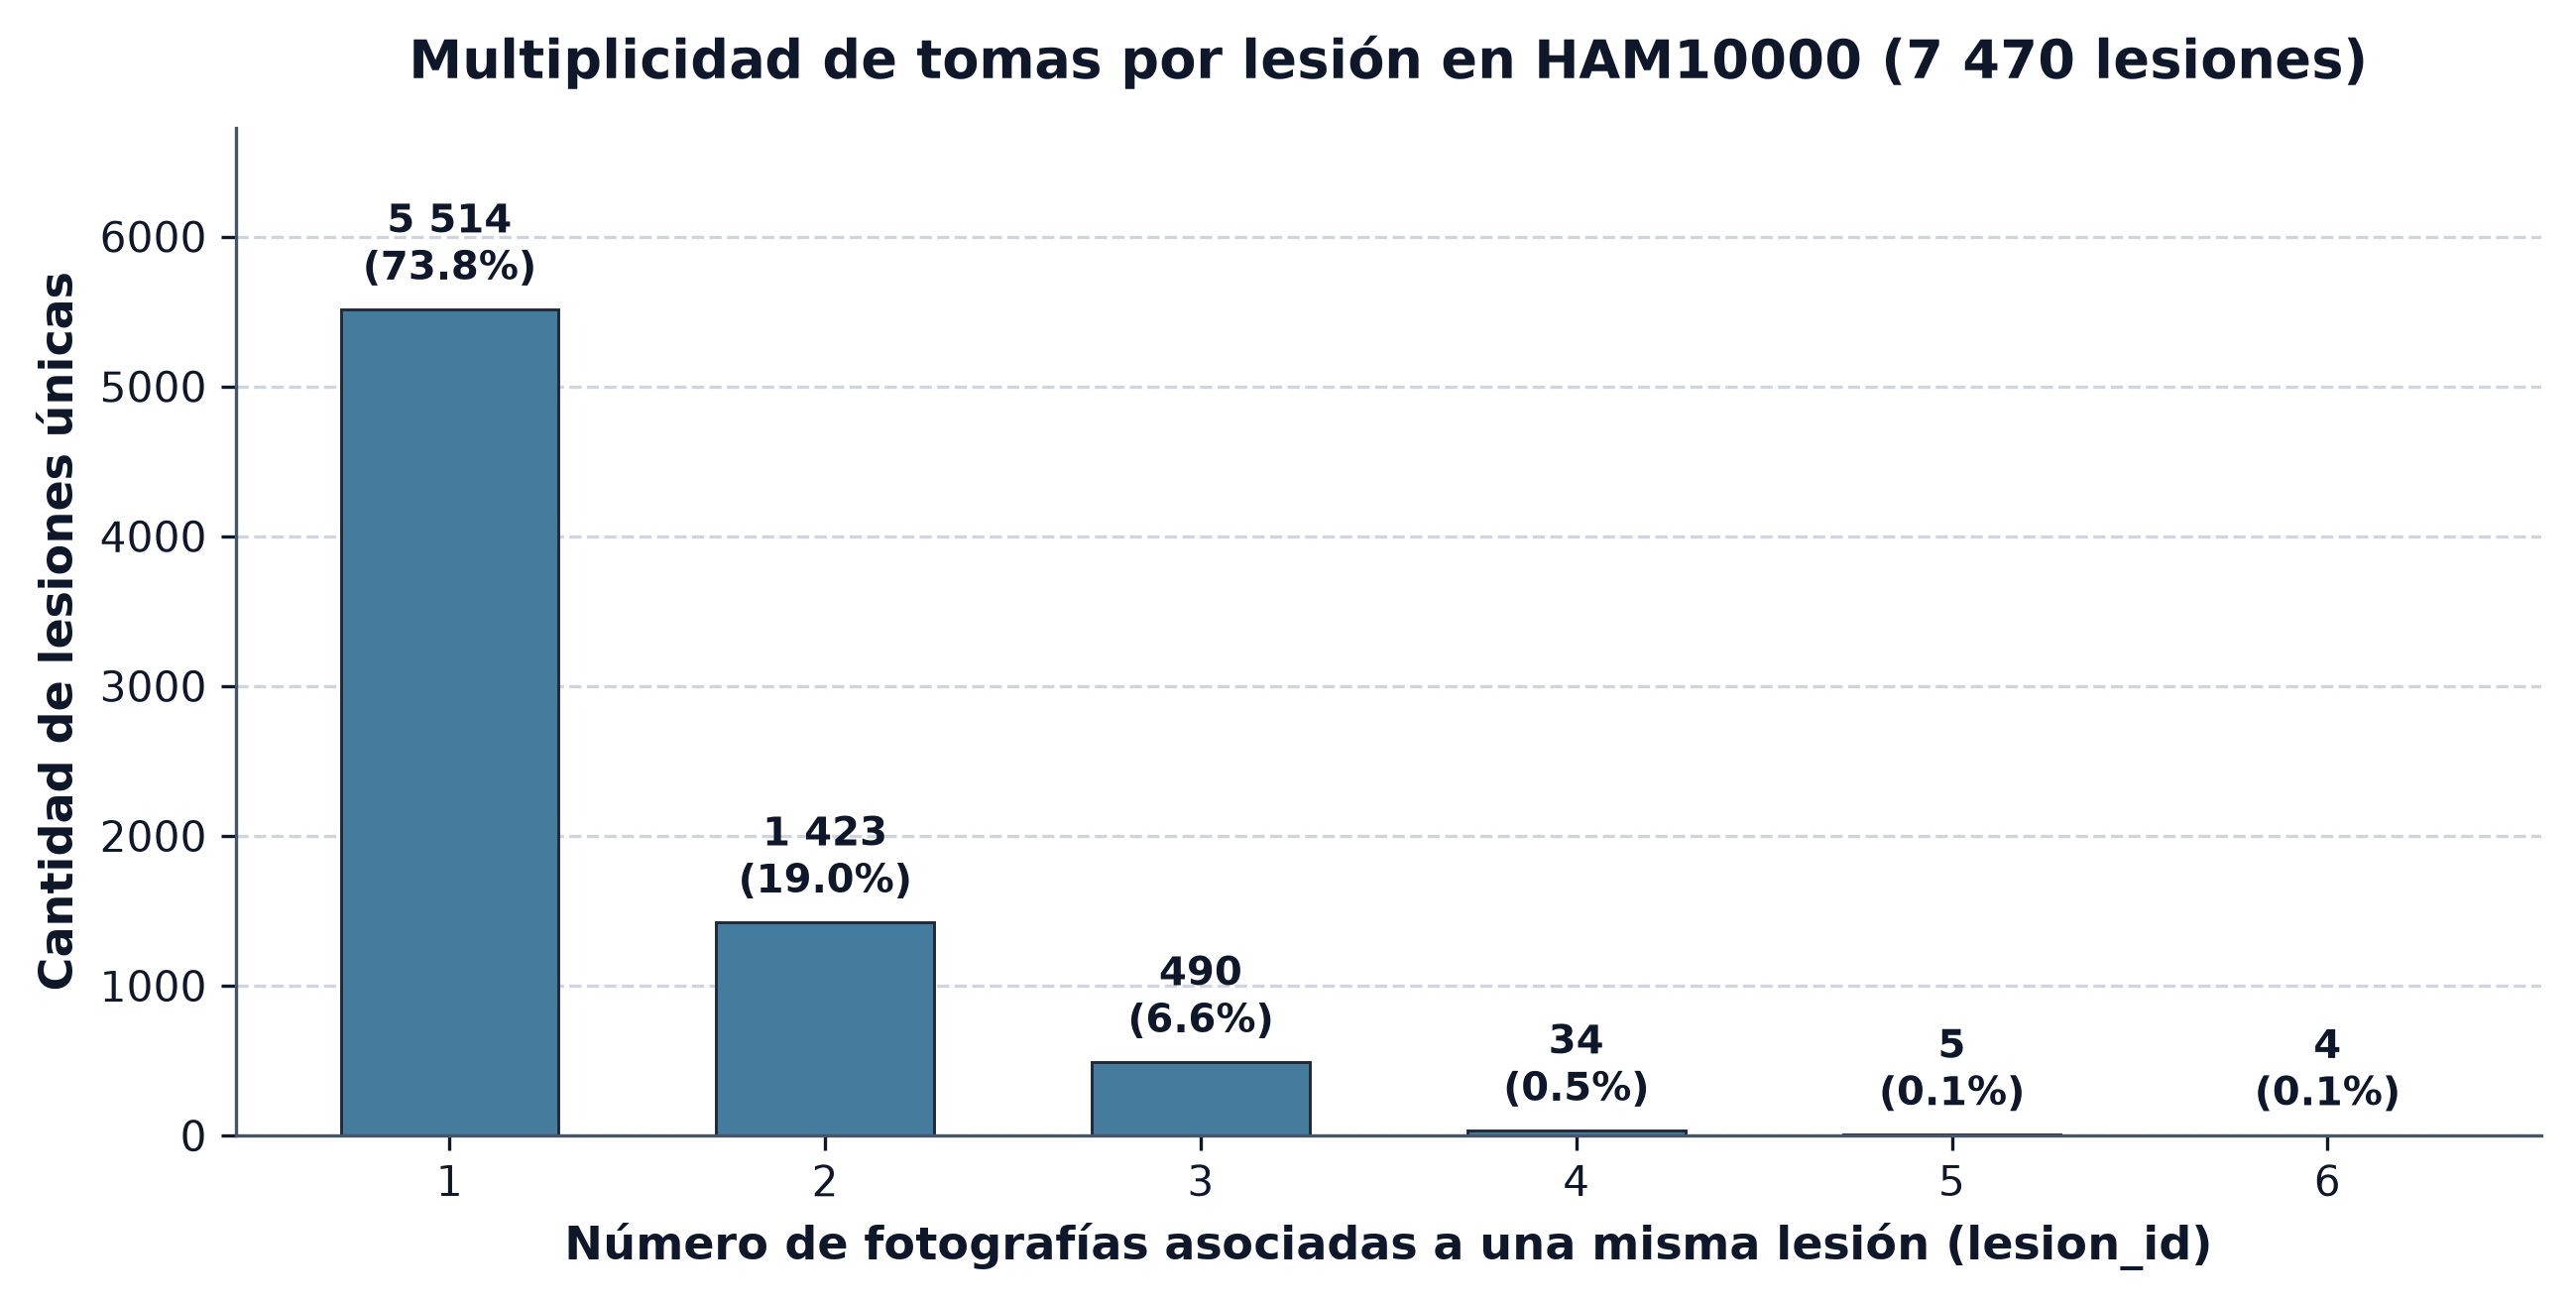
\includegraphics[width=0.92\textwidth]{05_multiplicidad.png}
\caption{Número de imágenes por lesión única (\texttt{lesion\_id}) en HAM10000 (26.2\% de las lesiones presentan múltiples tomas).}
\label{fig:multiplicidad}
\end{figure}

\begin{figure}[htbp]
\centering
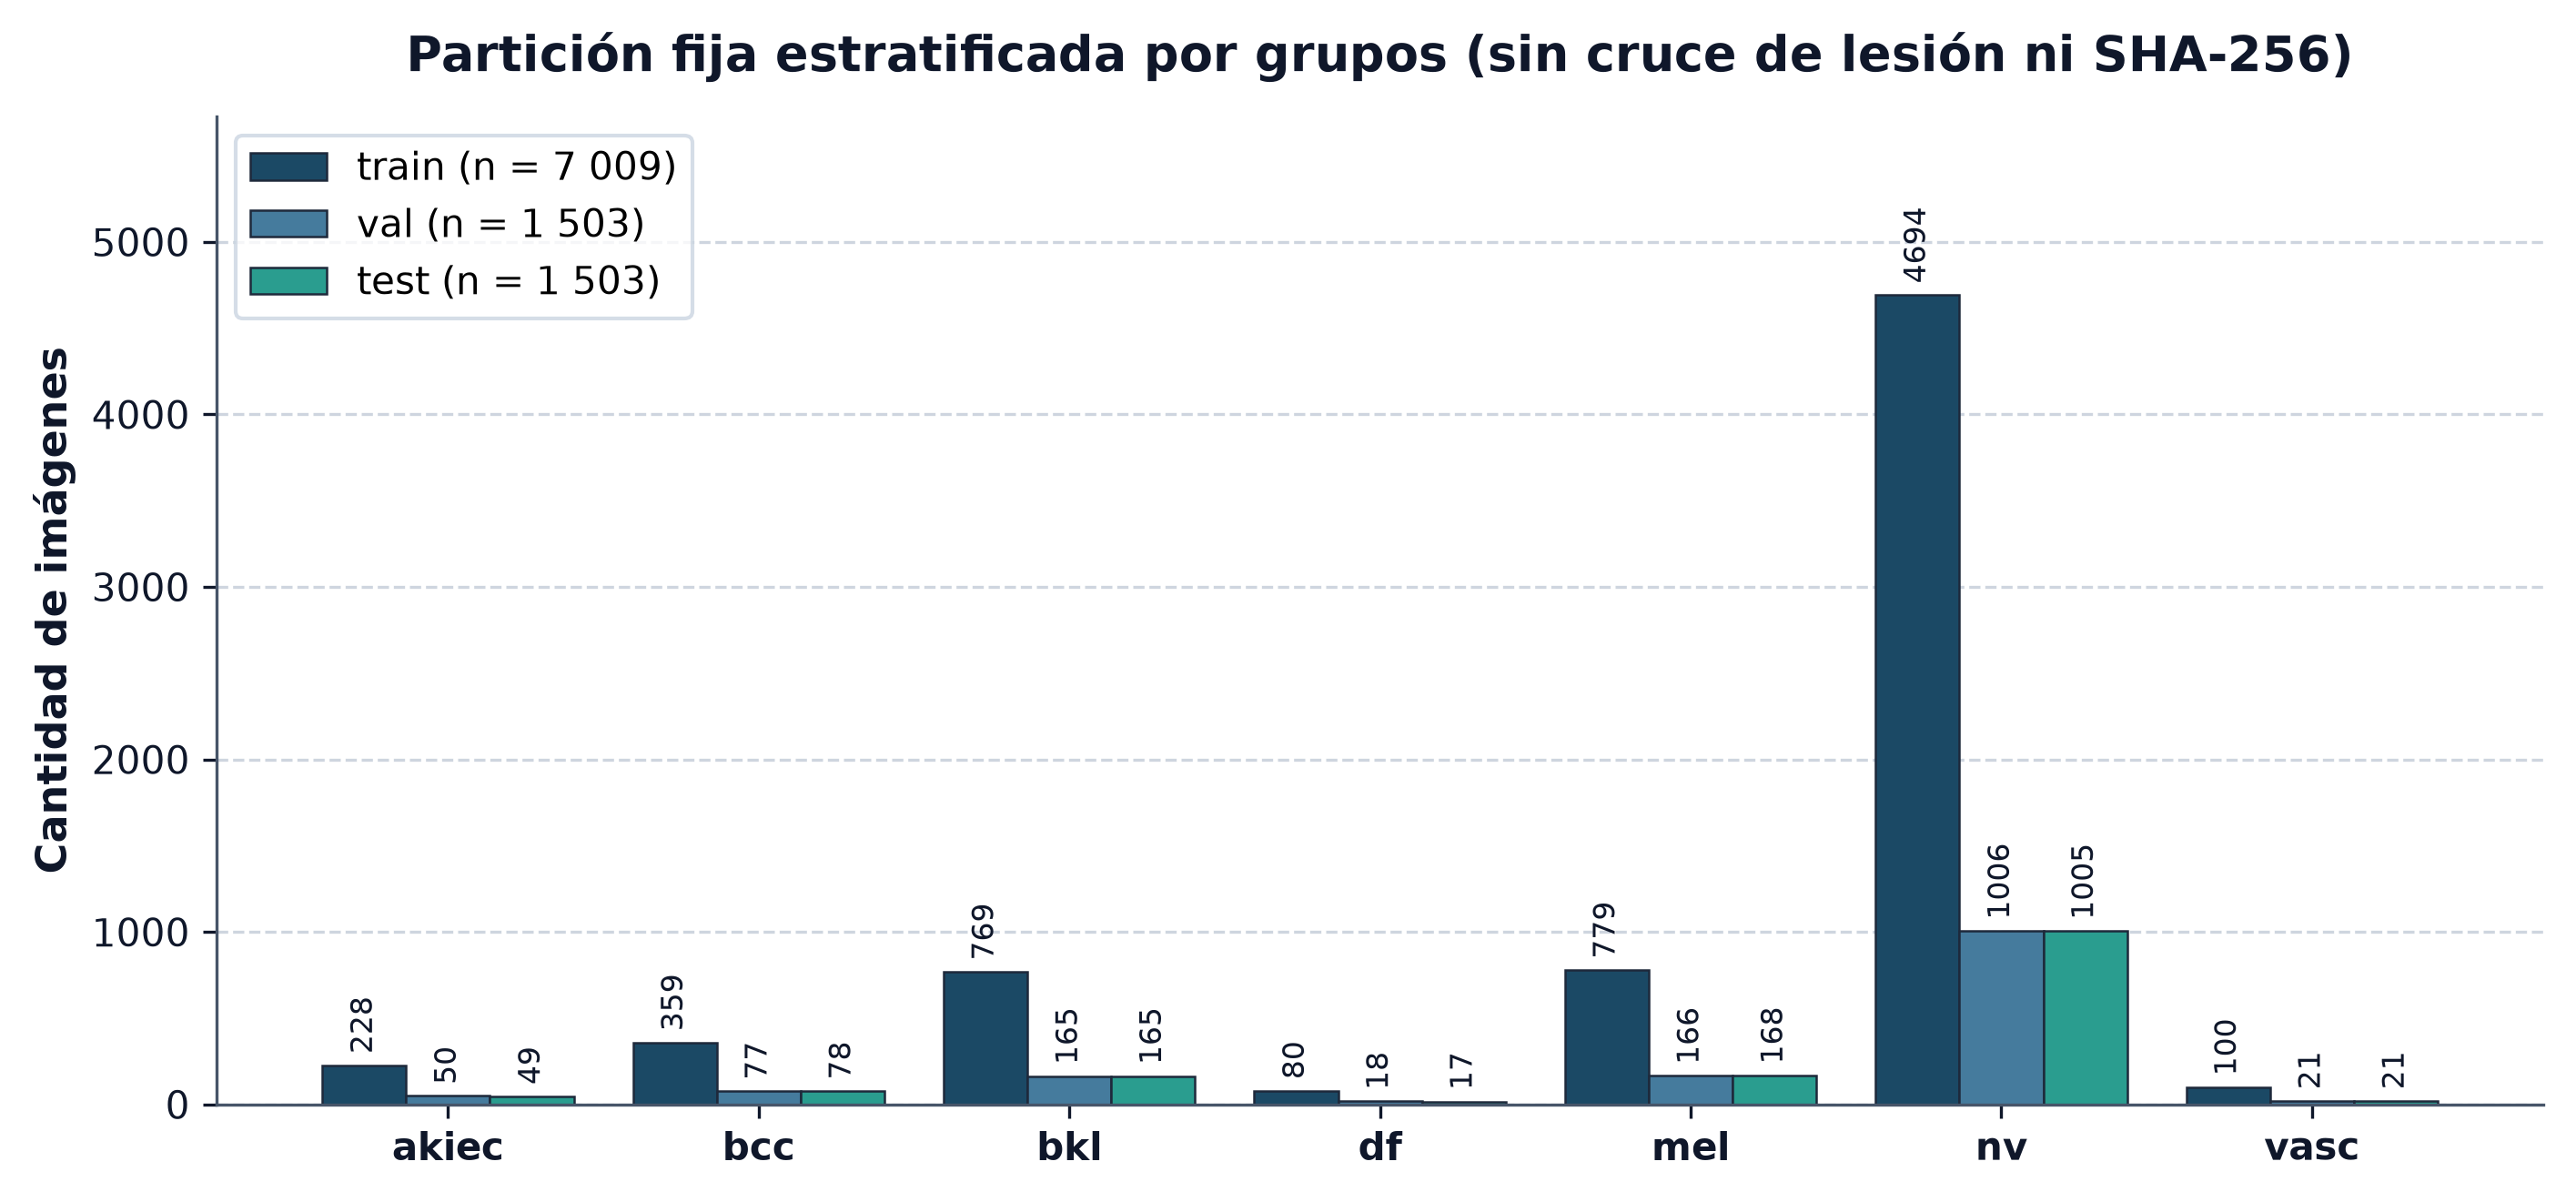
\includegraphics[width=0.92\textwidth]{04_split.png}
\caption{Conteos reales del split fijo por categoría diagnóstica en \texttt{train}, \texttt{val} y \texttt{test} tras agrupar por lesión y SHA-256 sin fugas.}
\label{fig:split}
\end{figure}
\FloatBarrier

\subsection{Pruebas automáticas de integridad y control criptográfico}
El programa verifica ausencia de cruce de \texttt{lesion\_id}, \texttt{group\_id} y SHA-256 entre particiones, exige presencia de todas las clases y conserva la huella del CSV completo. Los checkpoints guardan esa huella y rechazan una reanudación o evaluación con otro manifiesto. Al trasladar el proyecto a Colab se validan los 10\,015 archivos frente al mismo manifiesto sin volver a sortear el split.

\begin{table}[htbp]\centering\small
\caption{Resumen de verificaciones de integridad y control antifuga ejecutadas sobre \texttt{split.csv}.}
\begin{tabularx}{\textwidth}{@{}>{\bfseries\raggedright\arraybackslash}p{4.6cm}>{\raggedright\arraybackslash}p{4.6cm}>{\raggedright\arraybackslash}X@{}}
\toprule
\textbf{Comprobación} & \textbf{Resultado verificado} & \textbf{Mecanismo en \texttt{prepare.py} / \texttt{io.py}} \\ \midrule
Integridad archivo--metadata & 10\,015 / 10\,015 JPEG válidos & Verificación de lectura, dimensiones $600\times450$ y SHA-256. \\
Duplicados binarios exactos & 2 pares en \texttt{nv} confinados & Agrupación \textit{Union-Find} por \texttt{lesion\_id} + SHA-256 (7\,470 grupos). \\
Casi-duplicados entre lesiones & 0 pares con $\mathrm{RMSE} < 4.5$ (sesión) & Comprobación puntual de sesión en RGB $16\times12$ (sin reporte independiente; limitación perceptual vigente en \texttt{auditoria.json}). \\
Cruce entre subconjuntos & 0 intersecciones en 3 ejes & Aserciones de disjunción por lesión, grupo y SHA-256. \\
Inmutabilidad del manifiesto & \texttt{583779fb75f28758...} & Comprobación estricta de \texttt{split\_sha256} al reanudar o evaluar. \\
\bottomrule
\end{tabularx}
\end{table}
\FloatBarrier
